\section{Porównanie skuteczności systemu detekcji}
\subsection{Rozpatrywane metody standaryzacji danych}
\label{minimen}
Rozpatrzono skuteczność modelu wybranego przez MetaOD dla czterech metody standaryzacji danych oraz danych nieprzekształconych.
Rozpatrywane metody skalowania:
\begin{itemize}
    \item StandardScaler: standaryzacja Z wykorzystująca średnią oraz odchylenie standardowe cechy:\begin{equation}
        z=\frac{x-\mu}{\sigma}. 
    \end{equation}
    \item RobustScaler: standaryzacja odporna na obserwacje odstające, wykorzystuje medianę oraz rozstęp ćwiartkowy cechy:
    \begin{equation}
            X_{std}=\frac{X-mediana(X)}{IQR}
    \end{equation}
    
    \item MinMaxScaler: standaryzacja danych do przedziału [0,1], gdzie minimalna i maksymalna wartość cechy wyznaczają granice przedziału  \begin{equation}
    \label{mms}
        X_{std} = \frac{X - X_{min}}{X_{max} - X_{min}}
    \end{equation}    
    \item PowerTransformer (transformacja Yeo–Johnson \cite{yeo2000new}): transformacja symetryzująca rozkład zmiennej losowej. Dzięki czemu rozkład zmiennej losowej (cecha zbioru danych) przypomina rozkład normalny.
    \begin{equation}
    y_i^{(\lambda)} = \begin{cases} ((y_i+1)^\lambda-1)/\lambda                      &  \text{jeśli }\lambda \neq 0, y \geq 0 \\ 
                                \log(y_i + 1)                                    &  \text{jeśli }\lambda =    0, y \geq 0 \\ 
                                -[(-y_i + 1)^{(2-\lambda)} - 1] / (2 - \lambda)  &  \text{jeśli }\lambda \neq 2, y <    0 \\ 
                                -\log(-y_i + 1)                                  &  \text{jeśli }\lambda =    2, y <    0 
                  \end{cases}
    \end{equation}
\end{itemize}
% \begin{sidewaystable}
%     \centering
\begin{table}[]
    \centering
\begin{tabularx}{\textwidth}{lXXXXX}
      Zbiór & Dane oryginalne & Robust Scaler & Standard Scaler & MinMax Scaler & Power Transformer \\ \hline
arrhythmia &               0.7480 &                  0.7527 &            0.7685 &      0.8093 &      0.7619 \\
    cardio &               0.5474 &                  0.6150 &            0.8604 &      0.9109 &      0.3830 \\
     glass &               0.6249 &                  0.4016 &            0.7122 &      0.7518 &      0.6076 \\
ionosphere &               0.8336 &                  0.8308 &            0.8065 &      0.8678 &      0.8481 \\
    letter &               0.8790 &                  0.8096 &            0.8976 &      0.8411 &      0.9062 \\
    lympho &               0.9977 &                  0.9930 &            0.9953 &      0.9941 &      1.0000 \\
      musk &               0.9460 &                  0.9994 &            0.7267 &      0.9923 &      0.1024 \\
 optdigits &               0.7431 &                  0.4615 &            0.5380 &      0.4757 &      0.4856 \\
 pendigits &               0.6975 &                  0.7786 &            0.6792 &      0.7218 &      0.5707 \\
      pima &               0.6996 &                  0.7025 &            0.5650 &      0.6751 &      0.4289 \\
 satellite &               0.5549 &                  0.5394 &            0.6123 &      0.6380 &      0.3594 \\
satimage-2 &               0.9795 &                  0.9715 &            0.9688 &      0.9808 &      0.9469 \\
 vertebral &               0.3771 &                  0.7484 &            0.3465 &      0.2254 &      0.2835 \\
    vowels &               0.9551 &                  0.9727 &            0.9551 &      0.9543 &      0.9781 \\
       wbc &               0.8980 &                  0.8844 &            0.9689 &      0.8814 &      0.6293 \\
     mnist &               0.7737 &                  0.8051 &            0.6330 &      0.8130 &      0.6960 \\
   shuttle &               0.6166 &                  0.9860 &            0.6167 &      0.9973 &      0.6105 \\
\hline
Średnia &0.7572&
0.7795&
0.7442&
0.7959&
0.6234
\end{tabularx}
\caption{Porównanie skuteczności modelu wybranego przez MetaOD w zależności od metody standaryzacji danych -- pole pod krzywą ROC}
\footnotesize{źródło: Opracowanie własne}
\label{tab:roc_sc}
\end{table}
% \end{sidewaystable}
\begin{sidewaystable}
    \centering
\begin{tabular}{lrrrrr}
      Zbiór & Dane oryginalne & RobustScaler & StandardScaler & MinMaxScaler & PowerTransformer \\ \hline
arrhythmia &               0.3788 &                  0.4545 &            0.3788 &      0.4697 &      0.4242 \\
    cardio &               0.2273 &                  0.2159 &            0.4489 &      0.5114 &      0.1307 \\
     glass &               0.1111 &                  0.2222 &            0.1111 &      0.1111 &      0.0000 \\
ionosphere &               0.6349 &                  0.6429 &            0.6032 &      0.6984 &      0.6349 \\
    letter &               0.3800 &                  0.2600 &            0.5400 &      0.3100 &      0.4800 \\
    lympho &               0.8333 &                  0.6667 &            0.8333 &      0.8333 &      1.0000 \\
      musk &               0.6495 &                  0.9381 &            0.0309 &      0.7320 &      0.0515 \\
 optdigits &               0.0067 &                  0.0067 &            0.0733 &      0.0200 &      0.0400 \\
 pendigits &               0.0769 &                  0.0769 &            0.0705 &      0.0641 &      0.0513 \\
      pima &               0.5485 &                  0.5373 &            0.3881 &      0.5187 &      0.2985 \\
 satellite &               0.3723 &                  0.3900 &            0.5231 &      0.5373 &      0.1876 \\
satimage-2 &               0.8451 &                  0.8310 &            0.8732 &      0.8592 &      0.6056 \\
 vertebral &               0.0667 &                  0.2667 &            0.0000 &      0.0000 &      0.0000 \\
    vowels &               0.5400 &                  0.7000 &            0.5400 &      0.6000 &      0.7200 \\
       wbc &               0.2857 &                  0.5714 &            0.6190 &      0.5714 &      0.1429 \\
     mnist &               0.3500 &                  0.3600 &            0.2314 &      0.4100 &      0.2557 \\
   shuttle &               0.1925 &                  0.8762 &            0.4000 &      0.9425 &      0.1837 \\
\hline
Średnia &0.3823&
0.4716&
0.392&
0.4817&
0.3063

\end{tabular}
    \caption{Porównanie skuteczności modelu wybranego przez MetaOD w zależności od metody standaryzacji danych -- P@N}
    \footnotesize{źródło: Opracowanie własne}
    \label{tab:pn_sc}
\end{sidewaystable}


% \subsection{da}
\begin{sidewaystable}
    \centering
\begin{tabular}{lrrrrrrrrrr}
\toprule
      Zbiór &  \#Obserwacji &  \# Cech &  \% Anomalii &   ABOD &   HBOS &  IForest &    KNN &    LOF &  OCSVM &  MetaOD \\
\midrule
arrhythmia &       452 &           274 &       14.6018 & 0.7688 & 0.8219 &   0.8005 & 0.7861 & 0.7787 & 0.7812 &  0.8093 \\
    cardio &      1831 &            21 &        9.6122 & 0.5692 & 0.8351 &   0.9213 & 0.7236 & 0.5736 & 0.9348 &  0.9109 \\
     glass &       214 &             9 &        4.2056 & 0.7951 & 0.7389 &   0.7569 & 0.8508 & 0.8644 & 0.6324 &  0.7518 \\
ionosphere &       351 &            33 &       35.8974 & 0.9248 & 0.5614 &   0.8499 & 0.9267 & 0.8753 & 0.8419 &  0.8678 \\
    letter &      1600 &            32 &        6.2500 & 0.8783 & 0.5927 &   0.6420 & 0.8766 & 0.8594 & 0.6118 &  0.8411 \\
    lympho &       148 &            18 &        4.0541 & 0.9110 & 0.9957 &   0.9941 & 0.9745 & 0.9771 & 0.9759 &  0.9941 \\
     mnist &      7603 &           100 &        9.2069 & 0.7815 & 0.5742 &   0.8159 & 0.8481 & 0.7161 & 0.8529 &  0.8130 \\
      musk &      3062 &           166 &        3.1679 & 0.1844 & 1.0000 &   0.9999 & 0.7986 & 0.5287 & 1.0000 &  0.9923 \\
 optdigits &      5216 &            64 &        2.8758 & 0.4667 & 0.8732 &   0.7253 & 0.3708 & 0.4500 & 0.4997 &  0.4757 \\
 pendigits &      6870 &            16 &        2.2707 & 0.6878 & 0.9238 &   0.9435 & 0.7486 & 0.4698 & 0.9303 &  0.7218 \\
      pima &       768 &             8 &       34.8958 & 0.6794 & 0.7000 &   0.6806 & 0.7078 & 0.6271 & 0.6215 &  0.6751 \\
 satellite &      6435 &            36 &       31.6395 & 0.5714 & 0.7581 &   0.7022 & 0.6836 & 0.5573 & 0.6622 &  0.6380 \\
satimage-2 &      5803 &            36 &        1.2235 & 0.8190 & 0.9804 &   0.9947 & 0.9536 & 0.4577 & 0.9978 &  0.9808 \\
   shuttle &     49097 &             9 &        7.1511 & 0.6234 & 0.9855 &   0.9971 & 0.6537 & 0.5264 & 0.9917 &  0.9973 \\
 vertebral &       240 &             6 &       12.5000 & 0.4262 & 0.3263 &   0.3905 & 0.3817 & 0.4081 & 0.4431 &  0.2254 \\
    vowels &      1456 &            12 &        3.4341 & 0.9606 & 0.6727 &   0.7585 & 0.9680 & 0.9410 & 0.7802 &  0.9543 \\
       wbc &       378 &            30 &        5.5556 & 0.9047 & 0.9516 &   0.9310 & 0.9366 & 0.9349 & 0.9319 &  0.8814 \\
\bottomrule
 Średnia & & & &
0.7031&
0.7819&
0.8179&
0.7758&
0.6792&
0.7935&
0.7959&
\end{tabular}
\caption{Porównanie pola pod krzywą ROC wybranego modelu przez MetaOD do modeli PyOD}
\footnotesize{źródło: Opracowanie własne na podstawie \cite{zhao2019pyod}}
    \label{tab:roc_od}
\end{sidewaystable}

\begin{sidewaystable}
    \centering
\begin{tabular}{lrrrrrrrrrr}
\toprule
       Zbiór &  \#Obserwacji &  \# Cech &  \% Anomalii &   ABOD &   HBOS &  IForest &    KNN &    LOF &  OCSVM &  MetaOD \\
\midrule
arrhythmia &       452 &           274 &       14.6018 & 0.3808 & 0.5111 &   0.4961 & 0.4464 & 0.4334 & 0.4614 &  0.4697 \\
    cardio &      1831 &            21 &        9.6122 & 0.2374 & 0.4476 &   0.5041 & 0.3323 & 0.1541 & 0.5011 &  0.5114 \\
     glass &       214 &             9 &        4.2056 & 0.1702 & 0.0000 &   0.0726 & 0.0726 & 0.1476 & 0.1726 &  0.1111 \\
ionosphere &       351 &            33 &       35.8974 & 0.8442 & 0.3295 &   0.6369 & 0.8602 & 0.7063 & 0.7000 &  0.6984 \\
    letter &      1600 &            32 &        6.2500 & 0.3801 & 0.0715 &   0.1003 & 0.3312 & 0.3641 & 0.1510 &  0.3100 \\
    lympho &       148 &            18 &        4.0541 & 0.4483 & 0.8467 &   0.9267 & 0.7517 & 0.7517 & 0.7517 &  0.8333 \\
     mnist &      7603 &           100 &        9.2069 & 0.3555 & 0.1188 &   0.3135 & 0.4204 & 0.3343 & 0.3962 &  0.4100 \\
      musk &      3062 &           166 &        3.1679 & 0.0507 & 0.9783 &   0.9680 & 0.2733 & 0.1695 & 1.0000 &  0.7320 \\
 optdigits &      5216 &            64 &        2.8758 & 0.0060 & 0.2194 &   0.0301 & 0.0000 & 0.0234 & 0.0000 &  0.0200 \\
 pendigits &      6870 &            16 &        2.2707 & 0.0812 & 0.2979 &   0.3422 & 0.0984 & 0.0653 & 0.3287 &  0.0641 \\
      pima &       768 &             8 &       34.8958 & 0.5193 & 0.5424 &   0.5111 & 0.5413 & 0.4555 & 0.4704 &  0.5187 \\
 satellite &      6435 &            36 &       31.6395 & 0.3902 & 0.5690 &   0.5676 & 0.4994 & 0.3893 & 0.5346 &  0.5373 \\
satimage-2 &      5803 &            36 &        1.2235 & 0.2130 & 0.6939 &   0.8754 & 0.3809 & 0.0555 & 0.9356 &  0.8592 \\
   shuttle &     49097 &             9 &        7.1511 & 0.1977 & 0.9551 &   0.9546 & 0.2184 & 0.1424 & 0.9542 &  0.9425 \\
 vertebral &       240 &             6 &       12.5000 & 0.0601 & 0.0071 &   0.0343 & 0.0238 & 0.0506 & 0.0238 &  0.0000 \\
    vowels &      1456 &            12 &        3.4341 & 0.5710 & 0.1297 &   0.1875 & 0.5093 & 0.3551 & 0.2791 &  0.6000 \\
       wbc &       378 &            30 &        5.5556 & 0.3060 & 0.5817 &   0.5088 & 0.4952 & 0.5188 & 0.5125 &  0.5714 \\
\bottomrule
 Średnia & & & &0.3066&
0.4294&
0.4723&
0.3679&
0.301&
0.4808&
0.4817&
\end{tabular}
\caption{Porównanie P@N wybranego modelu przez MetaOD do modeli PyOD}
\footnotesize{źródło: Opracowanie własne na podstawie \cite{zhao2019pyod}}
\end{sidewaystable}



\begin{sidewaysfigure}
    \centering
    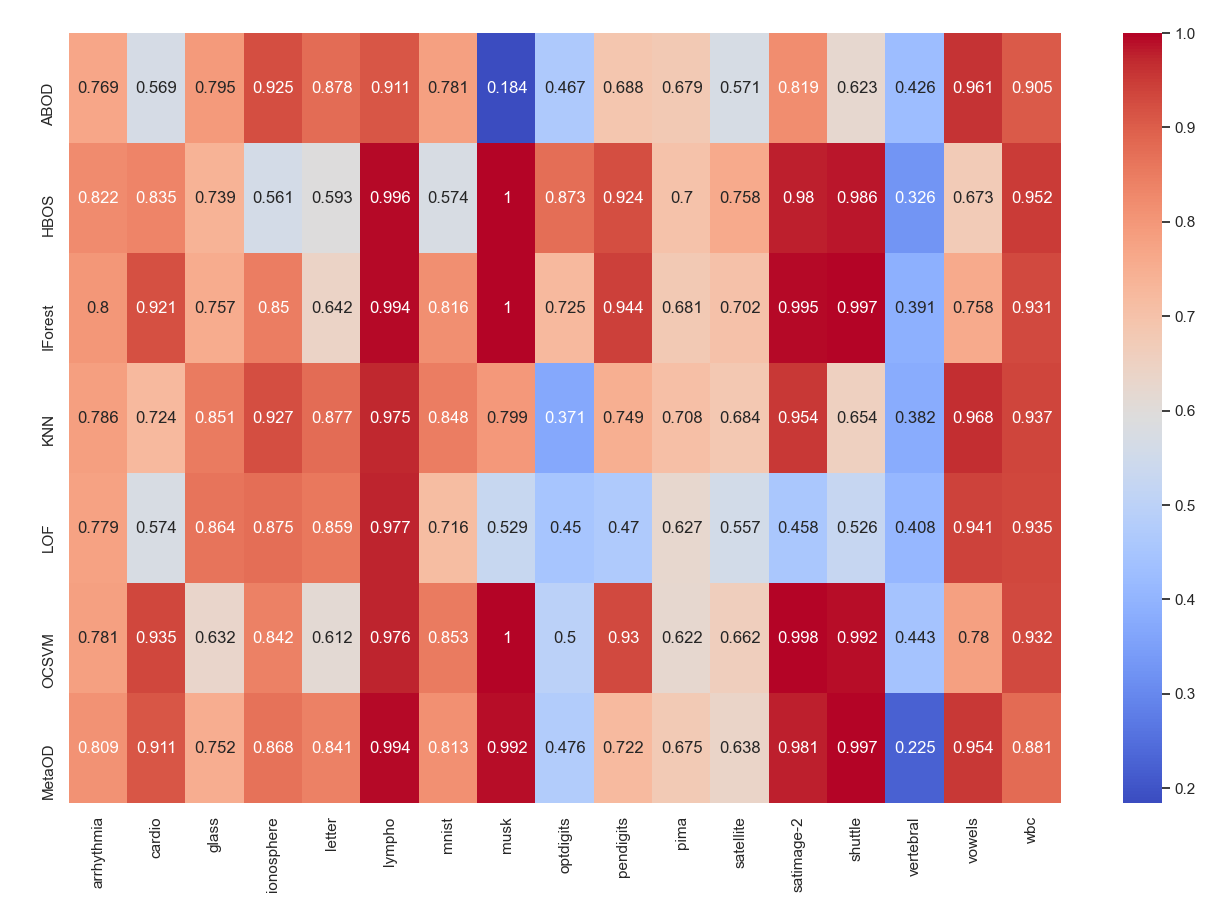
\includegraphics[width = \textwidth]{chapters/analiza/img/roc.png}
    \caption{Mapa ciepła pola pod krzywą ROC}
    \footnotesize{źródło: Opracowanie własne }
    \label{fig:h1}
\end{sidewaysfigure}


\begin{sidewaysfigure}
    \centering
    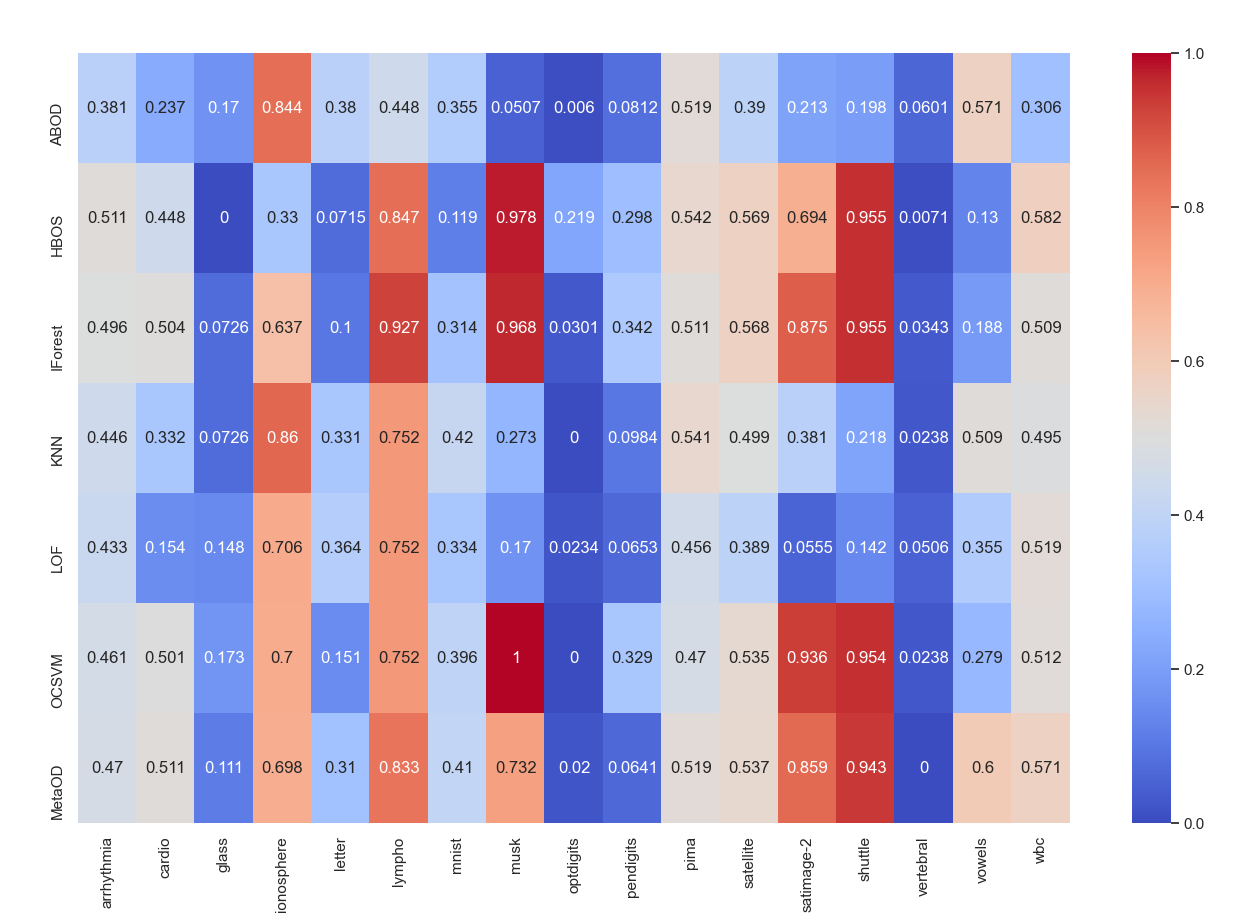
\includegraphics[width =\textwidth]{chapters/analiza/img/prc.png}
    \caption{Mapa ciepła P@N}
    \footnotesize{źródło: Opracowanie własne }
    \label{fig:h2}
 \end{sidewaysfigure}

\section{Analiza wyników}
Na podstawie wyników z badania skuteczności metody standaryzacji danych (Tabela \ref{tab:roc_sc} oraz \ref{tab:pn_sc}) zdecydowano na standaryzację danych, wykorzystując MinMaxScaler. Standaryzacja  danych z wykorzystaniem MinMaxScaler zwiększyła średnią skuteczność wybranego modelu w porównaniu do modelu wybranego na podstawie danych niepoddanych standaryzacji o:
\begin{itemize}
    \item średnie pole pod krzywą ROC: wzrosło o 5,11\%
    \item średnie P@N: wzrosło o 26\%
\end{itemize}
W wyniku standaryzacji danych wykorzystując MinMaxScaler, MetaOD skutecznością zajęło -- w porównaniu do algorytmów PyOD -- odpowiednio: 
\begin{itemize}
    \item Na podstawie średniego pola pod krzywą ROC: 2 miejsce -- lepsza skuteczność: \textit{Isolation Forest} 
    \item Na podstawie średniego P@N: 1 miejsce 
\end{itemize}

Mapy ciepła dla P@N i pola pod krzywą ROC (Rysunek \ref{fig:h1} i \ref{fig:h2}) pokazują, że wybrany model przez MetaOD dla zbiorów danych, dla których inne modele były nieskuteczne, również jest nieskuteczny (zbiór danych: vertebral). Jednakże porównując średnią wartość P@N oraz pola pod krzywą ROC model wybrany przez MetaOD wyróżnia się skutecznością detekcji na tle innych modeli, wraz z algorytmem \textit{Isolation Forest}. Analizując wyniki, dochodzimy do konkluzji, że początkowe rozwiązanie wykorzystujące algorytm \textit{Isolation Forest} byłoby porównywalnie skuteczne co wybrana metoda wykorzystująca meta-uczenie. 

Jednak podczas analizy porównawczej skuteczności modeli wybranych przez MetaOD w zależności od metody standaryzacji danych można zaobserwować, iż wybór skutecznej metody standaryzacji dla konkretnego zbioru danych może znacząco podnieść skuteczność detekcji anomalii, np. model wybrany po standaryzacji danych wykorzystując RobustScaler dla zbioru \textit{vertebral}. Otwiera to możliwość badań nie tylko nad wyborem modelu, ale również metody standaryzacji oraz transformacji danych.
